\documentclass[11pt,a4paper]{article}
\usepackage[utf8]{inputenc}
\usepackage{amsmath, amssymb}
\usepackage{geometry}
\usepackage{listings}
\usepackage{xcolor}
\usepackage{ctex}
\usepackage{graphicx}
\usepackage{algorithm}
\usepackage{algpseudocode}
\usepackage{subcaption}

% 设置页面边距
\geometry{top=2.5cm, bottom=2.5cm, left=2.5cm, right=2.5cm}

\title{实验报告:三维环境设计与展示}
\author{董奕柳}
\date{\today}

\begin{document}

\maketitle

\section{实验目的}
设计一个三维环境,并利用 OpenGL 展示其三维效果,要求:
\begin{itemize}
    \item 包含基本的实体元素:球、多面体、锥体、柱体、曲面等;
    \item 实现全局光照效果和纹理功能;
    \item 程序具有交互功能。
\end{itemize}

通过实验,熟悉 OpenGL 的基本用法和三维图形的绘制技巧,掌握光照和纹理处理技术,以及基本的交互编程能力。

\section{实验环境}
\begin{itemize}
    \item 开发语言:C++
    \item 图形库:OpenGL
    \item 开发工具:Visual Studio Code + MinGW
    \item 操作系统:Windows
\end{itemize}

\section{设计与实现}

\subsection{总体设计}
在本实验中,三维环境包含以下部分:
\begin{itemize}
    \item 基本几何体:球、多面体、锥体、柱体、曲面等;
    \item 光照效果:实现环境光、漫反射光和镜面反射光;
    \item 纹理功能:为部分几何体添加纹理;
    \item 交互功能:通过键盘或鼠标实现视角切换和物体控制。
\end{itemize}

\subsection{功能模块设计}
\subsubsection{几何体绘制模块}
实现以下几何体的绘制:
\begin{itemize}
    \item 球体:基于 OpenGL 的 \texttt{glutSolidSphere} 和 \texttt{glutWireSphere} 实现,分别展示实体和线框效果。
    \begin{figure}[h]
        \centering
        \includegraphics[width=0.4\textwidth]{sphere.png}
        \caption{球体渲染效果}
    \end{figure}
    
    \item 立方体:使用 \texttt{glutSolidCube} 和 \texttt{glutWireCube} 绘制实心和线框立方体。
    \begin{figure}[h]
        \centering
        \includegraphics[width=0.4\textwidth]{cube.png}
        \caption{立方体渲染效果}
    \end{figure}

    \item 锥体:通过 \texttt{glutSolidCone} 和 \texttt{glutWireCone} 实现锥体的实体和线框效果。
    \begin{figure}[h]
        \centering
        \includegraphics[width=0.4\textwidth]{cone.png}
        \caption{锥体渲染效果}
    \end{figure}

    \item 圆环:通过 \texttt{glutSolidTorus} 和 \texttt{glutWireTorus} 实现。
    \begin{figure}[h]
        \centering
        \includegraphics[width=0.4\textwidth]{torus.png}
        \caption{圆环渲染效果}
    \end{figure}

    \item 正多面体:绘制如十二面体(\texttt{glutSolidDodecahedron} 和 \texttt{glutWireDodecahedron})、八面体、四面体、二十面体等。
    \begin{figure}[h]
        \centering
        \includegraphics[width=0.4\textwidth]{dodecahedron.png}
        \caption{正十二面体渲染效果}
    \end{figure}

    \item 茶壶模型:使用 \texttt{glutSolidTeapot} 和 \texttt{glutWireTeapot} 绘制经典的 OpenGL 茶壶。
    \begin{figure}[h]
        \centering
        \includegraphics[width=0.4\textwidth]{teapot.png}
        \caption{茶壶模型渲染效果}
    \end{figure}
\end{itemize}

\subsubsection{光照与纹理模块}
\begin{itemize}
    \item 光照:配置全局光源和局部光源,利用 OpenGL 提供的光照模型实现,其中包括 \texttt{glLightfv} 用于设置光源参数(环境光、散射光和镜面光),\texttt{glEnable} 用于启用光源,\texttt{glMaterialfv} 和 \texttt{glColorMaterial} 用于设置材质属性;
    \begin{figure}[h]
        \centering
        % 左图
        \begin{subfigure}[b]{0.45\textwidth}
            \centering
            \includegraphics[width=\textwidth]{teapot1.png}
            \caption{茶壶1}
            \label{fig:teapot_no_light}
        \end{subfigure}
        \hfill
        % 右图
        \begin{subfigure}[b]{0.45\textwidth}
            \centering
            \includegraphics[width=\textwidth]{teapot2.png}
            \caption{茶壶2}
            \label{fig:teapot_with_light}
        \end{subfigure}
        % 总标题
        \caption{不同光照效果下的茶壶对比}
        \label{fig:teapot_light_comparison}
    \end{figure}


    \item 纹理:加载图片作为纹理,通过 \texttt{SOIL\_load\_OGL\_texture} 加载纹理文件,利用 \texttt{glTexParameteri} 配置纹理的过滤和环绕模式,并使用 \texttt{gluQuadricTexture} 将纹理映射到几何体表面(如球体的地球效果)。

    \begin{figure}[H]
        \centering
        \begin{minipage}{0.3\textwidth}
            \centering
            \includegraphics[width=\textwidth]{world_map.png}
            \caption*{(a) 二维世界地图}
        \end{minipage}
        \hfill
        \begin{minipage}{0.3\textwidth}
            \centering
            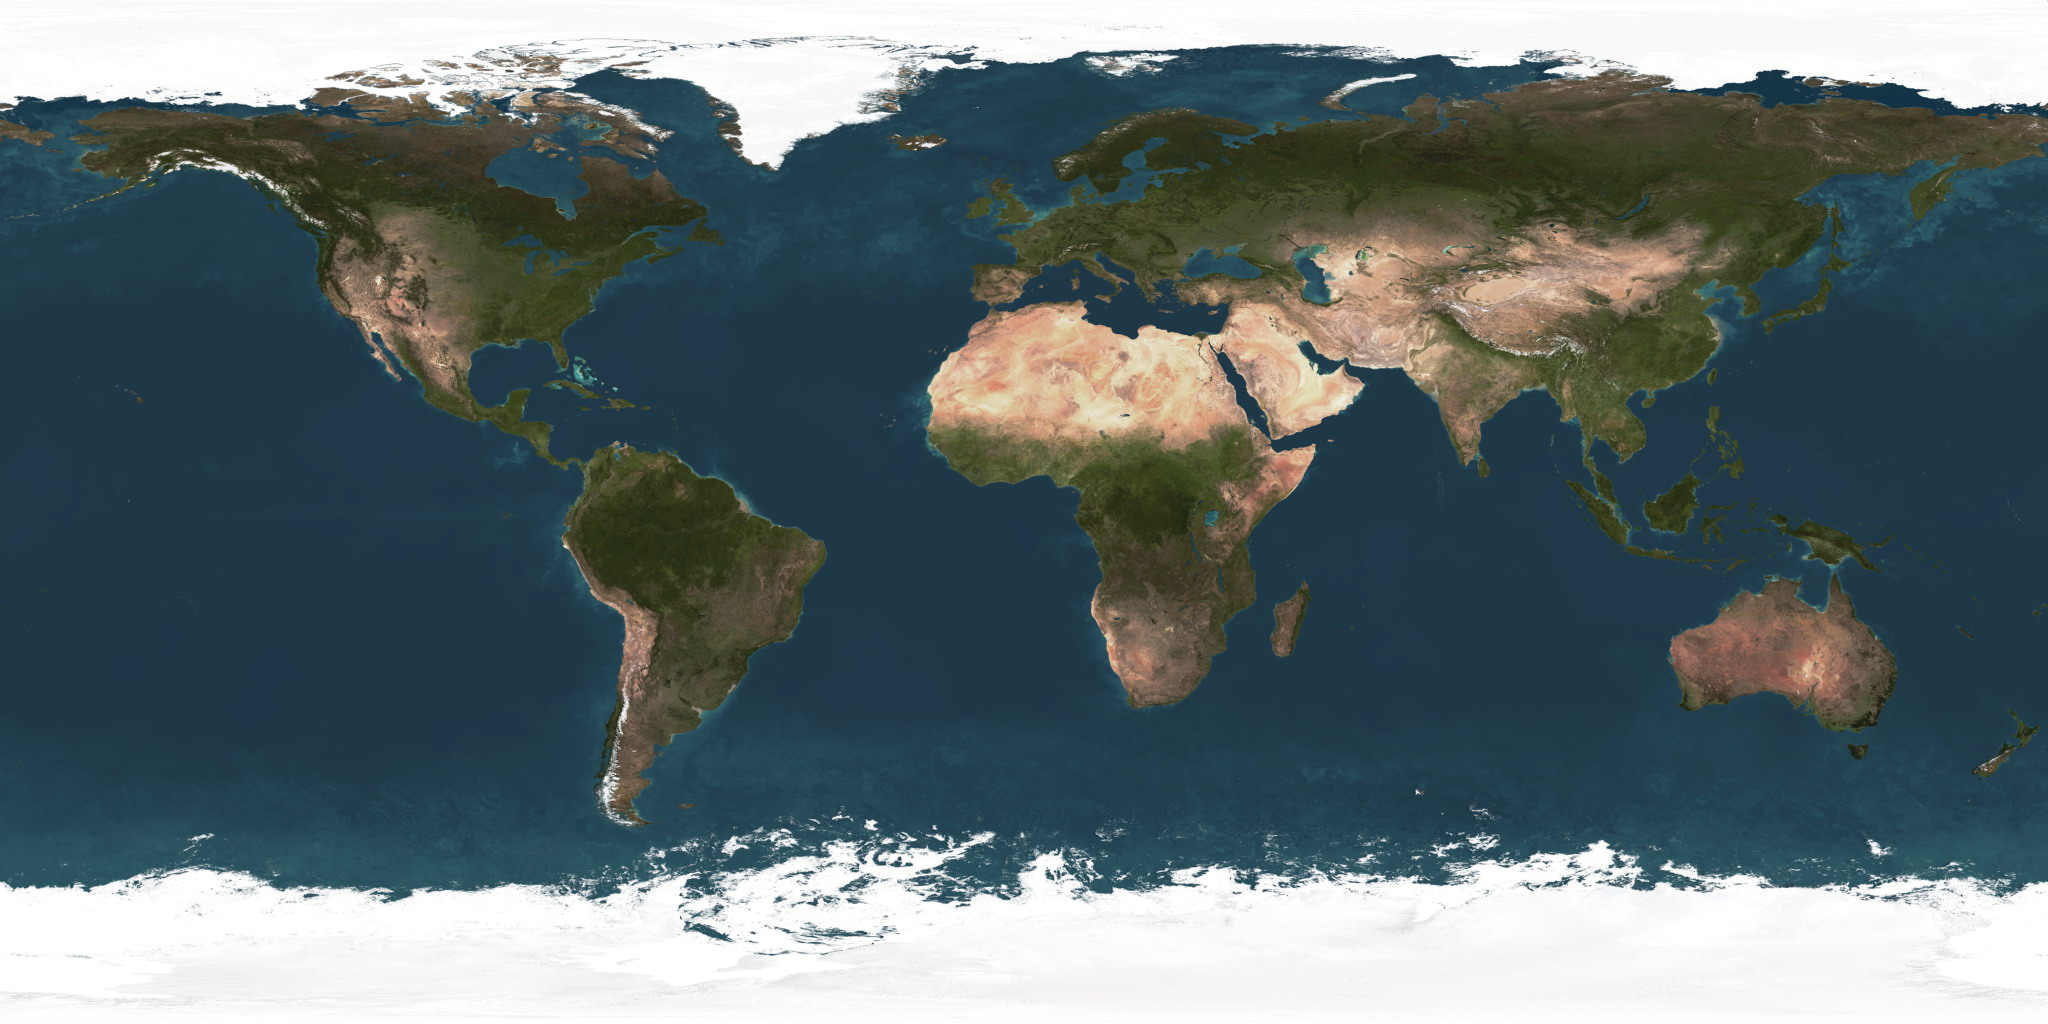
\includegraphics[width=\textwidth]{earth.png}
            \caption*{(b) 赤道视角地球}
        \end{minipage}
        \hfill
        \begin{minipage}{0.3\textwidth}
            \centering
            \includegraphics[width=\textwidth]{earth2.png}
            \caption*{(c) 北极视角地球}
        \end{minipage}
        \caption{纹理的球体映射:二维世界地图被映射到三维球体,且球体上的像素是连续的。}
        \label{fig:texture_comparison}
    \end{figure}


\end{itemize}

\subsubsection{交互模块}
通过以下方式实现程序的交互功能:
\begin{itemize}
    \item \textbf{键盘交互}:使用 \texttt{WASD} 键控制光源位置的上下左右移动,使用方向键实现视角的旋转;
    \item \textbf{鼠标交互}:通过鼠标右键唤出菜单,可以更改物体形状、光照配置或纹理参数;
\end{itemize}


\section{实验结果}

本节展示实验的主要结果,包括各功能模块的运行效果。实验结果通过图片和简单文字说明进行描述。

\subsection{功能一:房屋显示效果}
\begin{figure}[H]
    \centering
    \begin{subfigure}[b]{0.32\textwidth}
        \centering
        \includegraphics[width=\textwidth]{house_close.png} % 近观图的路径
        \caption{近观效果}
        \label{fig:house_close}
    \end{subfigure}
    \hfill
    \begin{subfigure}[b]{0.32\textwidth}
        \centering
        \includegraphics[width=\textwidth]{house.png} % 远观图的路径
        \caption{远观效果}
        \label{fig:house_far}
    \end{subfigure}
    \hfill
    \begin{subfigure}[b]{0.32\textwidth}
        \centering
        \includegraphics[width=\textwidth]{house_perspective.png} % 透视图的路径
        \caption{透视效果}
        \label{fig:house_perspective}
    \end{subfigure}
    \caption{房屋模型的显示效果,包括近观、远观和透视图。}
    \label{fig:house_display}
\end{figure}

\subsection{功能二:光照效果}
\begin{figure}[H]
    \centering
    \begin{subfigure}[b]{0.48\textwidth}
        \centering
        \includegraphics[width=\textwidth]{light_on.png} % 光照开启的图片路径
        \caption{光照开启效果}
        \label{fig:light_on}
    \end{subfigure}
    \hfill
    \begin{subfigure}[b]{0.48\textwidth}
        \centering
        \includegraphics[width=\textwidth]{light_off.png} % 光照关闭的图片路径
        \caption{光照关闭效果}
        \label{fig:light_off}
    \end{subfigure}
    \caption{光照效果对比,左图为光照开启,右图为光照关闭。}
    \label{fig:light_effect}
\end{figure}

\subsection{功能三:交互功能}
\begin{figure}[H]
    \centering
    \includegraphics[width=\textwidth]{menu.png} % 请替换为实际的图片路径
    \caption{菜单交互功能展示。图中显示了菜单的界面以及其功能选项。}
    \label{fig:menu_interaction}
\end{figure}


以上实验结果验证了系统各功能模块的正确性与可用性。



\section{总结}
通过本次实验,我实现了一个基本的三维环境,包括几何体绘制、全局光照与纹理功能,以及简单的交互功能。实验中,我熟悉了 OpenGL 的基本绘图流程和光照、纹理的实现方法,掌握了三维环境的设计思路和技术实现。

\end{document}
